\documentclass[journal,12pt,onecolumn]{IEEEtran}
% Page configurations
\usepackage[a4paper,bottom=1in,top=1in]{geometry}
\usepackage{amsmath}
\usepackage{graphicx}
\usepackage{float}
\usepackage{tikz}
\usepackage{multicol}
\setlength{\columnsep}{1cm}
% \usepackage{gvv-book}
\usepackage{gvv}
\usetikzlibrary{arrows}
\usetikzlibrary{decorations.markings}
\graphicspath{{figs/}}
\usepackage{amsmath}
\usepackage{amssymb}
\usepackage{geometry}
\geometry{margin=1in}
%\usepackage{gvv}

\begin{document}

\title{
GATE ASSIGNMENT}
\author{AI25BTECH11015 - M Sai Rithik}
\maketitle


\section*{Geomatics Engineering (GE) \\ General Aptitude (GA)}

\textbf{Q.1 -- Q.5 Carry ONE mark Each}



\begin{enumerate}
    \item "You are delaying the completion of the task. Send \underline{\hspace{2cm}} contributions at the earliest."

    A. you are \quad
    B. your \quad
    C. you're \quad
    D. yore

    \item References : \_\_\_\_ : : Guidelines : Implement (By word meaning)

    A. Sight \quad
    B. Site \quad
    C. Cite \quad
    D. Plagiarise

    \item In the given figure, PQRS is a parallelogram with $PS=7$ cm, $PT=4$ cm and $PV=5$ cm. What is the length of $RS$ in cm? (The figure is representative.)

    A. $\frac{20}{7}$ \quad
    B. $\frac{28}{5}$ \quad
    C. $\frac{9}{2}$ \quad
    D. $\frac{35}{4}$

    \begin{figure}[h] 
    \centering
    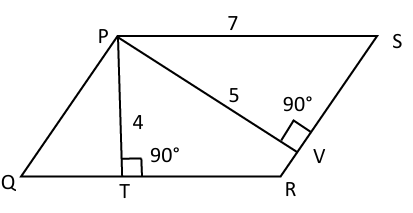
\includegraphics[width=0.5\textwidth]{figs/qn3.png}
    \caption{Parallelogram}
\label{fig:q3 graph}
\end{figure}



\begin{center}

\end{center}

    \item In 2022, June Huh was awarded the Fields medal, which is the highest prize in Mathematics. When he was younger, he was also a poet. He did not win any medals in the International Mathematics Olympiads. He dropped out of college.

    Based only on the above information, which one of the following statements can be logically inferred with certainty?

    A. Every Fields medalist has won a medal in an International Mathematics Olympiad. \\
    B. Everyone who has dropped out of college has won the Fields medal. \\
    C. All Fields medalists are part-time poets. \\
    D. Some Fields medalists have dropped out of college.

    \item A line of symmetry is defined as a line that divides a figure into two parts in a way such that each part is a mirror image of the other part about that line. The given figure consists of 16 unit squares arranged as shown. In addition to the three black squares, what is the minimum number of squares that must be coloured black, such that both $PQ$ and $MN$ form lines of symmetry? (The figure is representative)

    A. 3 \quad
    B. 4 \quad
    C. 5 \quad
    D. 6

    \begin{figure}[h] 
    \centering
    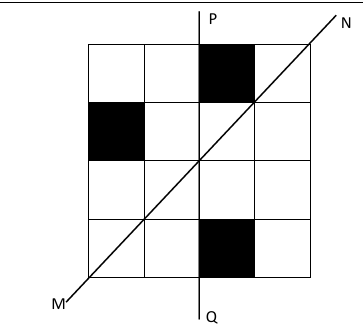
\includegraphics[width=0.5\textwidth]{figs/qn5.png}
    \caption{}
\label{fig:q5graph}
\end{figure}

\begin{center}
\end{center}

\end{enumerate}

\textbf{Q.6 -- Q.10 Carry TWO marks Each}

\begin{enumerate}
    \setcounter{enumi}{5}
    \item Human beings are one among many creatures that inhabit an imagined world. In this imagined world, some creatures are cruel. If in this imagined world, it is given that the statement “Some human beings are not cruel creatures” is FALSE, then which of the following set of statement(s) can be logically inferred with certainty?

    (i) All human beings are cruel creatures. \\
    (ii) Some human beings are cruel creatures. \\
    (iii) Some creatures that are cruel are human beings. \\
    (iv) No human beings are cruel creatures.

    A. only (i) \\
    B. only (iii) and (iv) \\
    C. only (i) and (ii) \\
    D. (i), (ii) and (iii)

    \item To construct a wall, sand and cement are mixed in the ratio of 3:1. The cost of sand and that of cement are in the ratio of 1:2. If the total cost of sand and cement to construct the wall is 1000 rupees, then what is the cost (in rupees) of cement used?

    A. 400 \quad
    B. 600 \quad
    C. 800 \quad
    D. 200

    \item The World Bank has declared that it does not plan to offer new financing to Sri Lanka, which is battling its worst economic crisis in decades, until the country has an adequate macroeconomic policy framework in place. In a statement, the World Bank said Sri Lanka needed to adopt structural reforms that focus on economic stabilisation and tackle the root causes of its crisis. The latter has starved it of foreign exchange and led to shortages of food, fuel, and medicines. The bank is repurposing resources under existing loans to help alleviate shortages of essential items such as medicine, cooking gas, fertiliser, meals for children, and cash for vulnerable households.

    Based only on the above passage, which one of the following statements can be inferred with certainty?

    A. According to the World Bank, the root cause of Sri Lanka’s economic crisis is that it does not have enough foreign exchange. \\
    B. The World Bank has stated that it will advise the Sri Lankan government about how to tackle the root causes of its economic crisis. \\
    C. According to the World Bank, Sri Lanka does not yet have an adequate macroeconomic policy framework. \\
    D. The World Bank has stated that it will provide Sri Lanka with additional funds for essentials such as food, fuel, and medicines.

    \item The coefficient of $x^4$ in the polynomial $(x-1)^3(x-2)^3$ is equal to \rule{3cm}{0.15mm}.

    A. 33 \quad
    B. $-3$ \quad
    C. 30 \quad
    D. 21

    \item Which one of the following shapes can be used to tile (completely cover by repeating) a flat plane, extending to infinity in all directions, without leaving any empty spaces in between them? The copies of the shape used to tile are identical and are not allowed to overlap.

    A. circle \quad
    B. regular octagon \quad
    C. regular pentagon \quad
    D. rhombus
\end{enumerate}

\textbf{Q.11 -- Q.31 Carry ONE mark Each}

\begin{enumerate}
    \setcounter{enumi}{10}
    \item An angle was measured with a standard error of 5ʺ. How many observations a surveyor needs to take in order to obtain a standard error of 1ʺ for the mean value of this angle?

    A. 5 \quad
    B. 1 \quad
    C. 10 \quad
    D. 25

    \item What are the Manhattan and Pythagorean distances (in m), respectively between points A and B in the figure below, where the Euclidean distance between A and C is 4 m, and the Euclidean distance between C and B is 4 m? All the cells have the same edge lengths.

\begin{center}

\end{center}

    A. 9.0 and 5.7 \quad
    B. 5.7 and 8.0 \quad
    C. 5.7 and 5.7 \quad
    D. 8.0 and 5.7

\begin{figure}[h] 
    \centering
    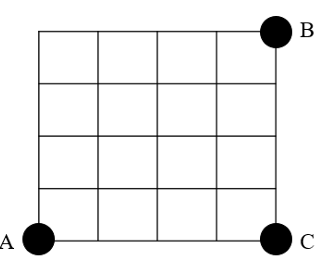
\includegraphics[width=0.5\textwidth]{figs/qn12.png}
    \caption{Figure}
\label{fig:q12graph}
\end{figure}

    \item Which of the following is tested using the Chi-square test in least squares adjustment?

    A. Adjusted and observed values of observations are statistically similar \\
    B. Presence of gross errors in observations \\
    C. Adjusted and assumed values of parameters are statistically similar \\
    D. High correlation between observations and residuals

    \item In active remote sensing of Earth objects from a satellite-borne sensor, the source of the energy used for sensing, lies at the \rule{3cm}{0.15mm}.

    A. satellite \quad
    B. Sun \quad
    C. object being sensed on Earth \quad
    D. ground station

    \item For a push-broom sensor, the following details are given: \\
    Number of detectors = 3000 \\
    Height above the ground = 900 km \\
    Swath on the ground = 30 km \\  
    The spatial resolution of the sensor is \rule{3cm}{0.15mm} m.

    A. 30 \quad
    B. 270 \quad
    C. 3 \quad
    D. 10

    \item To visually distinguish between a river channel and a canal on an image, having similar widths and located in the same area, the most important parameter used is \rule{3cm}{0.15mm}.

    A. size \quad
    B. shape \quad
    C. tone \quad
    D. texture

    \item The unit of spectral radiance is \rule{3cm}{0.15mm}.

    A. $W \, sr^{-1} \, \mu m^{-1}$ \quad
    B. $W \, m^{-2} \, sr^{-1}$ \quad
    C. $W \, m^{-2}$ \quad
    D. $W \, m^{-2} \, sr^{-1} \, \mu m^{-1}$

    \item The ratio between the reflected to the incident energy on a surface at a particular wavelength gives the \rule{3cm}{0.15mm} of the surface.

    A. spectral reflectance \quad
    B. spectral transmittance \quad
    C. spectral radiance \quad
    D. spectral irradiance

    \item GNSS stands for Global Navigation Satellite Systems. As of today, which of the following is the complete set of GNSS constellations that cover the entire globe?

    A. GPS, GLONASS, Galileo, BeiDou, IRNSS, QZSS \\
    B. GPS, GLONASS, Galileo, BeiDou, IRNSS, QZSS, GAGAN, WAAS, EGNOS \\
    C. GPS, GLONASS, Galileo \\
    D. GPS, GLONASS, Galileo, BeiDou

    \item The basic premise for using the DGPS technique is to reduce the errors due to

    A. atmosphere, satellite orbit, multipath \\
    B. atmosphere, satellite orbit, satellite clock \\
    C. atmosphere, satellite clock, receiver clock \\
    D. atmosphere, satellite orbit, satellite clock, receiver clock, multipath

    \item The orbital period of GPS satellites is determined by the \rule{3cm}{0.15mm} of their orbits.

    A. semi-major axis \quad
    B. eccentricity \quad
    C. inclination \quad
    D. semi-major axis, inclination and eccentricity

    \item Which vector data analysis tool combines geometries and attributes from different layers?

    A. Overlay \quad
    B. Map Manipulation \quad
    C. Buffer \quad
    D. Cartesian distance measurement

    \item A GIS analyst has two raster datasets with the same number of rows and columns. The analyst computes the average of the two input raster layers to generate a new raster layer with the same size as the input raster layers. What type of raster data analysis operation is performed?

    A. Local \quad
    B. Neighborhood \quad
    C. Zonal \quad
    D. Global
\end{enumerate}

\section*{Geomatics Engineering (GE) \\ General Aptitude (GA)}

\textbf{Q.24 -- Q.45 Carry ONE mark Each}

\begin{enumerate}
    \setcounter{enumi}{23}
    \item Match the following errors (Column 1) in spatial data digitization with their descriptions (Column 2). \\
    \begin{tabular}{ll}
    (P) Mis-located entities & 1) Points, lines or boundary segments digitized twice \\
    (Q) Missing labels & 2) Points, lines or boundary segments digitized in wrong place \\
    (R) Artefacts of digitization & 3) Undershoots, overshoots, wrongly placed nodes, loops or spikes \\
    (S) Duplicate labels & 4) Undefined polygons \\
    (T) Duplicate entities & 5) Two or more identification labels for same polygon
    \end{tabular}

    A. P-2, Q-4, R-3, S-5, T-1 \\
    B. P-1, Q-2, R-3, S-5, T-4 \\
    C. P-2, Q-1, R-4, S-3, T-5 \\
    D. P-2, Q-4, R-3, S-1, T-5

    \item Which of the following statement(s) is/are TRUE for the least squares adjustment of observations?

    A. Observations have a Chi-square distribution \\
    B. Random errors in the observations are assumed to have a symmetrical distribution \\
    C. The positive and negative random observation errors are equally likely \\
    D. The adjusted parameters are independent of a priori reference variance

    \item Which of the following statement(s) is/are TRUE for the systematic errors?

    A. These can be corrected by applying a suitable mathematical model \\
    B. The least squares adjustment automatically removes unmodelled systematic errors \\
    C. These must be removed while or before applying the least squares adjustment \\
    D. Removal of gross errors automatically removes systematic errors

    \item In the following figure, A and B are fixed points with known plane rectangular coordinates. C and D are the new points in the control survey whose coordinates are to be determined. For this network, the surveyor has measured all 8 internal angles (1 to 8) and 5 sides BC, CD, DA, AC and BD. The value of redundancy (r) for the given figure will be equal to \rule{3cm}{0.15mm} (In integer).

\begin{center}
\end{center}

\begin{figure}[h] 
    \centering
    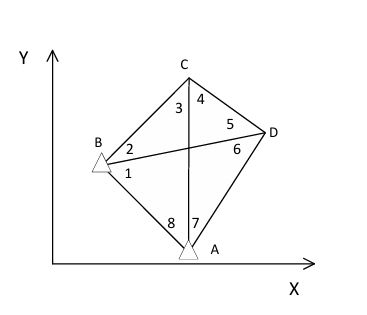
\includegraphics[width=0.5\textwidth]{figs/qn27.png}
    \caption{Graph}
\label{fig:q27}
\end{figure}

    \item As shown in the following figure, let $d_1, d_2, d_3$ denote three uncorrelated clockwise directions, observed at point P with equal standard errors for each direction, i.e., $\sigma_{d_1} = \sigma_{d_2} = \sigma_{d_3} = \pm \sqrt{2}''$. Let $\alpha_1$ and $\alpha_2$ be two included angles formed by these three directions. The covariance matrix (in arcsecond$^2$) for these included angles will be given as:

\begin{tabular}{rl}
P & $\alpha_1 \quad \alpha_2$ \\
$d_1$ & \\
$d_2$ & \\
$d_3$ & 
\end{tabular}

A. $\begin{bmatrix} 4 & 2 \\ 2 & 4 \end{bmatrix}$ \quad
B. $\begin{bmatrix} 4 & -2 \\ -2 & 4 \end{bmatrix}$ \\
C. $\begin{bmatrix} -4 & 2 \\ 2 & -4 \end{bmatrix}$ \quad
D. $\begin{bmatrix} 4 & 2 \\ -2 & 4 \end{bmatrix}$

\begin{figure}[h] 
    \centering
    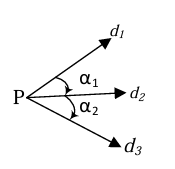
\includegraphics[width=0.5\textwidth]{figs/qn28.png}
    \caption{Diagram}
\label{fig:qn28}
\end{figure}

    \item The figure shows three distance observations $D_1$, $D_2$ and $D_3$. The table lists values of these observations and the corresponding weights. Assuming uncorrelated observations, the most probable values by the least squares approach for these measurements are ________ (Rounded off to 3 decimal places).

\begin{tabular}{lcc}
Distance Measurement (m) & Weight \\
$D_1$ & 40.150 & 1 \\
$D_2$ & 40.180 & 2 \\
$D_3$ & 80.390 & 1 \\
\end{tabular}

A. $\hat{D}_1=40.170$ m, $\hat{D}_2=40.190$ m, $\hat{D}_3=80.360$ m \\
B. $\hat{D}_1=40.174$ m, $\hat{D}_2=40.192$ m, $\hat{D}_3=80.366$ m \\
C. $\hat{D}_1=40.175$ m, $\hat{D}_2=40.185$ m, $\hat{D}_3=80.360$ m \\
D. $\hat{D}_1=40.172$ m, $\hat{D}_2=40.195$ m, $\hat{D}_3=80.367$ m

    \item Which of the following methods is widely used by the GNSS constellations to distinguish the satellites from each other at the GNSS receiver?

    A. Code Division Multiple Access (CDMA) \quad
    B. Time Division Multiple Access (TDMA) \quad
    C. Amplitude Division Multiple Access (ADMA) \quad
    D. Phase Division Multiple Access (PDMA)

    \item For the following data, the slope $m$ and intercept $c$ of the least squares fitted straight line $Y = mX + c$ are given as:

\begin{tabular}{ccc}
Point & $X$ & $Y$ \\
1 & 12 & 14 \\
2 & 14 & 16 \\
3 & 16 & 17 \\
\end{tabular}

A. Slope = 0.750, Intercept = 5.167 \\
B. Slope = 0.850, Intercept = 6.180 \\
C. Slope = 0.650, Intercept = 5.558 \\
D. Slope = 0.750, Intercept = 5.555
\end{enumerate}

\section*{Geomatics Engineering (GE) \\ General Aptitude (GA)}

\textbf{Q.32 -- Q.45 Carry TWO marks Each}

\begin{enumerate}
    \setcounter{enumi}{31}
    \item Which of the following statement(s) is/are CORRECT for sun-synchronous Earth observation satellites?

    A. They are in near-polar orbit around the Earth \\
    B. They cross the equator at different longitudes at nearly the same local solar time \\
    C. They maintain nearly the same sun-target-satellite geometry while crossing the equator at different longitudes \\
    D. The angle of inclination of their orbit is $< 1^\circ$

    \item Which of the following statement(s) is/are CORRECT?

    A. In optical remote sensing, more often we are interested in diffuse reflections \\
    B. The reflection will be diffuse if the incident wavelength is comparatively much larger than the surface roughness \\
    C. A surface that reflects microwave in specular manner may reflect the visible in diffuse manner \\
    D. All wavelengths emitted by the Sun reflect in diffuse manner from the objects on the surface of the Earth

    \item The spectral reflectance curves of three materials (A, B, and C) are shown in the figure below. Also shown are three wavelength bands at $X$, $Y$ and $Z$. Which of the following statement(s) is/are CORRECT?

    A. Each of the curve is the spectral signature of the respective material \\
    B. A sensor designed for the wavelength band ‘Y’ will best distinguish these materials in the image captured by the sensor \\
    C. A sensor designed for the wavelength band ‘Z’ will best distinguish these materials in the image captured by the sensor \\
    D. These curves are normally produced using a spectro-radiometer

    \item Which of the following statement(s) is/are TRUE?

    A. Topography is an example of continuous spatial feature \\
    B. Geo-relational data model stores spatial data and attribute data separately \\
    C. Object based data model stores spatial data and attribute data together \\
    D. Land surface temperature is an example of discrete spatial feature

    \item In the network shown below, after converting it to a topological graph, which of the following statement(s) is/are TRUE? (Assume there are no pseudo-nodes)

    A. The correct number of nodes (or vertices) are 7 \\
    B. The correct number of edges (or links) are 9 \\
    C. The total number of regions are 4 \\
    D. The correct number of edges (or links) are 8

    \item Which of the following type(s) of tolerances is/are used in editing GIS data?

    A. Snap tolerance \\
    B. Weed tolerance \\
    C. Grain tolerance \\
    D. Polygon tolerance

    \item Choose the CORRECT statement(s) regarding microwave remote sensing.

    A. Spatial resolution of passive microwave remote sensor is coarser than that of active microwave remote sensor from the same platform \\
    B. The intensity of signal returned by an object depends on its geometric as well as dielectric properties \\
    C. It is possible to “see through” the dense forest canopy using X-band active microwave remote sensing (i.e. signals can penetrate the dense forest canopy) \\
    D. Microwave remote sensing can be used in soil moisture studies

    \item Consider the Sun and the Earth as blackbodies at 6000 K and 300 K temperatures, respectively. Which of the following statement(s) is/are INCORRECT?

    A. Sun emits maximum energy at $9.3\, \mu m$ \\
    B. Sun does not emit energy at microwave \\
    C. The wavelengths of the energies emitted by the Sun are a sub-set of the wavelengths emitted by the Earth \\
    D. Earth does not emit energy at green wavelength

    \item Which of the following statement(s) concerning GNSS errors is/are CORRECT?

    A. Tropospheric delay increases with increasing relative humidity \\
    B. Ionospheric error is highly correlated with the position of the Moon \\
    C. Multipath error is caused by buildings and man-made features and not by vegetation \\
    D. The observed range is called as pseudorange because of its erroneous nature

    \item For a push-broom (along-track) sensor the following are known:

    Field of view (FoV) $= 2^\circ$ \\
    Instantaneous FoV $= 1$ milli-radian \\
    Time to scan one full scanline $= 2 \times 10^{-2}$ s \\
    Height above ground $= 100$ km \\
    The dwell time for a single pixel of this sensor is \rule{3cm}{0.15mm} s. (Rounded off to 2 decimal places)

    \item The range accuracy with a microsecond accurate clock in the GNSS receiver is about 300 m. If we improve the clock accuracy to $3.33 \times 10^{-x}$ s, the range accuracy becomes 1 cm. The value of $x$ is \rule{3cm}{0.15mm} (In integer). Assume the speed of light to be $c=3 \times 10^8$ m/s and that no other errors are being considered. (Hint: error-free range = speed of light $\times$ time of travel of the signal)

    \item A GPS satellite is flying at a distance of 20,000 km from the observer. The phase of the L1 carrier (1575.42 MHz) in degrees as received by the observer is \rule{3cm}{0.15mm} (Rounded off to 2 decimal places). Assume that the signal did not experience any refraction, reflection or other errors and the speed of light to be $c=3 \times 10^8$ m/s.

    \item For a profile given in the figure in the form of three steps $A$, $B$ and $C$, the following information is available:

    Height of step $A$ ($H_A$) with respect to a reference line $= 10$ m (known and error free) \\
    Difference in height between step $A$ and step $B$ ($h_1$) $= 5$ m $\pm$ 2 mm \\
    Difference in height between step $B$ and step $C$ ($h_2$) $= 8$ m $\pm$ 3 mm \\
    $H_B$ and $H_C$ are the unknown heights of step $B$ and $C$, respectively. The step $B$ is higher than step $C$ and $D$. \\
    The coefficient of correlation, $\rho_{h_1 h_2}$, between the height differences $= 0.25$. \\
    The coefficient of correlation between estimated heights of points $B$ and $C$ ($\rho_{H_B H_C}$) will be \rule{3cm}{0.15mm} (Rounded off to 2 decimal places).

    \item The relative radiance value of a facet of a Triangulated Irregular Network (TIN) can be computed using: \\
    $R_f = \cos(A_f - A_s) \sin(H_f) \cos(H_s) + \cos(H_f) \sin(H_s)$, \\
    where $R_f$ is the relative radiance value of a facet, $A_f$ is the facet’s aspect, $A_s$ is the sun’s azimuth angle, $H_f$ is the facet’s slope and $H_s$ is the sun’s altitude. \\
    Suppose a facet of a TIN has a slope value of $10^\circ$ and an aspect value of $297^\circ$ and sun’s azimuth of $315^\circ$. For sun’s altitude angle of $65^\circ$, the relative radiance value of this facet is \rule{3cm}{0.15mm} (Rounded off to 2 decimal places).
\end{enumerate}

\section*{Geomatics Engineering (GE) \\ General Aptitude (GA)}

\textbf{Q.46 -- Q.81 Carry TWO marks Each}

\begin{enumerate}
    \setcounter{enumi}{45}
    \item The table provides the $X$- and $Y$-coordinates of the points, measured in row and column of a raster with cell size of 1 meter, and their known values. Using inverse distance weighted (IDW) interpolation method and Euclidean distance, the interpolated value at Point 0 is \rule{3cm}{0.15mm} (Rounded to 2 decimal places). A constant rate of change in value between points should be assumed.

\begin{tabular}{cccc}
Point & $X$ & $Y$ & Value \\
1 & 69 & 76 & 27 \\
2 & 59 & 67 & 10 \\
3 & 74 & 79 & 13 \\
0 & 69 & 67 & ? \\
\end{tabular}

    \item The bearing of the line $AB$ from North is $143^\circ 40'$ and angle $ABC$ measured in clockwise direction is $309^\circ 30'$. The bearing of line $BC$ in Quadrantal Bearing System is \rule{3cm}{0.15mm}.

    A. N$3^\circ 10'$W \quad
    B. N$86^\circ 50'$E \quad
    C. N$86^\circ 50'$W \quad
    D. N$3^\circ 10'$E

    \item Which of the following map scale is most suitable for urban planning?

    A. 1:10,000 \quad
    B. 1:25,000 \quad
    C. 1:50,000 \quad
    D. 1:100,000

    \item Which of the following statement is NOT true regarding relief displacement in vertical photographs in the context of aerial photogrammetry?

    A. Relief displacement is the shift in the photographic position of an object caused by the elevation of the object (above or below the datum) \\
    B. Relief displacement is always in non-radial direction from the principal point \\
    C. Relief displacement can cause straight roads (not passing through the ground principal point) to appear crooked in undulating terrain \\
    D. The magnitude of relief displacement is affected by the flying height of the camera (assuming everything else to be same)

    \item A square grid is laid on a flat terrain and is photographed from an aerial camera. The flying height and camera parameters are assumed to be constant. The camera and lens are assumed to be perfect (i.e. free from any distortions). The image of the grid obtained from the camera is shown below. Select the CORRECT statement from the statements given below.

    A. Camera is looking directly downwards (towards nadir) \quad
    B. The given photograph is a vertical photograph \quad
    C. The given photograph is an oblique photograph \quad
    D. Scale over the given photograph is constant

\begin{figure}[h] 
    \centering
    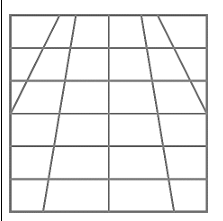
\includegraphics[width=0.5\textwidth]{figs/qn50.png}
    \caption{Diagram}
\label{fig:qn50}
\end{figure}
    \item Which of the following statement is TRUE for the World Geodetic System 1984 (WGS84)?

    A. The WGS84 ellipsoid best fits the shape of the earth including its topography \\
    B. The WGS84 ellipsoid and the Geodetic Reference System 1980 (GRS80) ellipsoid are one and the same \\
    C. The WGS84 ellipsoid is not a geocentric ellipsoid \\
    D. The WGS84 ellipsoid can be used to determine the geoid

    \item Which of the following map(s) is/are published by Survey of India?

    A. Topographical Maps \quad
    B. Geological Maps \quad
    C. Soil Maps \quad
    D. Thematic Maps

    \item Which of the following triangles are well conditioned and may be suitable for control establishment using triangulation?

\begin{tabular}{lc}
Triangle & Interior Angles \\
I & $90^\circ$, $45^\circ$, $45^\circ$ \\
II & $130^\circ$, $25^\circ$, $25^\circ$ \\
III & $110^\circ$, $35^\circ$, $35^\circ$ \\
IV & $110^\circ$, $45^\circ$, $25^\circ$ \\
\end{tabular}

    A. I \quad
    B. II \quad
    C. III \quad
    D. IV

    \item An angle of $90^\circ$ is to be laid out with a theodolite having a least count of $30''$. The angle was measured by repetition method and was found to be $90^\circ 00' 25''$. The offset value at a distance of 300 m from the theodolite to set-out the correct angle is \rule{3cm}{0.15mm} m (Rounded off to 3 decimal places).

    \item The following vertical circle readings were taken by a theodolite set up at station $A$ to observe targets located at $P$ and $Q$:

\begin{tabular}{lcccc}
Instrument at & Sighted to & Observation-1 (Vernier C) & Observation-1 (Vernier D) & Observation-2 (Vernier C) & Observation-2 (Vernier D) \\
$A$ & $P$ & $3^\circ 10' 10''$ & $10' 20''$ & $3^\circ 10' 30''$ & $10' 50''$ \\
$A$ & $Q$ & $-2^\circ 40' 40''$ & $41' 00''$ & $-2^\circ 41' 20''$ & $41' 10''$ \\
\end{tabular}

The value of the vertical angle $PAQ$ is \rule{3cm}{0.15mm}.

    \item Aerial photograph is to be taken from a flying height of 2 km above a flat ground with a camera having a focal length of 200 mm. The image format used is $23\,cm \times 23\,cm$. The ground area covered by a single photograph is \rule{3cm}{0.15mm} $km^2$.

    A. 5.29 \quad
    B. 1.48 \quad
    C. 0.95 \quad
    D. 2.22

    \item The scaled and rotated versions of vectors $[1, 2]$ and $[-3, 4]$ are \rule{3cm}{0.15mm}.

    A. $[-1, 3]$, $[-7,1]$ \quad
    B. $[5, 7]$, $[-7, 3]$ \quad
    C. $[2, -3]$, $[-7, 1]$ \quad
    D. $[2, -3]$, $[-7, 3]$

    \item Find the best match between Column 1 and Column 2:

\begin{tabular}{ll}
P: Trilateration & 1. Measurements of lengths and directions of all sides \\
Q: Triangulation & 2. Measurements of all the sides of a triangle \\
R: Traversing & 3. Measurements of all the interior angles of a triangle \\
S: Resection & 4. Determination of occupied position with the help of known stations \\
\end{tabular}

    A. P – 4; Q – 2; R – 3; S – 1 \\
    B. P – 1; Q – 3; R – 2; S – 4 \\
    C. P – 4; Q – 3; R – 2; S – 1 \\
    D. P – 2; Q – 3; R – 1; S – 4

    \item Which of the following statement(s) is/are CORRECT?

    A. WGS84 ellipsoid is an oblate ellipsoid \\
    B. GPS positioning gives the orthometric height of a place \\
    C. Height of a point above the geoid is its ellipsoidal height \\
    D. Shape of geoid changes with time

    \item For a constant flying height, the average scale of an aerial photograph depends on which of the following parameter(s)?

    A. Focal length of the camera \quad
    B. Size of the photograph \quad
    C. Size of the objects in the area \quad
    D. Topography of the ground

    \item Which of the following statement(s) is/are CORRECT?

    A. Mean sea level is defined as the long-term mean of the tide gauge measurements at a given location \\
    B. Mean sea level is the same as the mean tide level \\
    C. Mean sea level is defined as the monthly mean of the tide gauge measurements \\
    D. Mean sea level is an approximation of geoid

    \item Following is the page of a field book used for levelling. Few readings marked with ‘-’ are illegible. The Reduced Level (RL) of the Temporary Bench Mark (TBM) is \rule{3cm}{0.15mm} m (Rounded off to 2 decimal places). All the readings are in m.

    \item The zone number of Universal Transverse Mercator (UTM) projection having a longitude of $67^\circ 20' 30''$E is \rule{3cm}{0.15mm} (In integer).

    \item A pair of overlapping vertical photographs were taken from a flying height of 1230 m above sea level with a camera having a focal length of 152.4 mm. The distance between the consecutive exposure stations is 350 m. The parallax bar reading of a point A on the photograph is observed as 10.96 mm. The parallax bar constant for this setup is given as 80.71 mm. The elevation of point A above sea level is found to be \rule{3cm}{0.15mm} m (Rounded off to 2 decimal places).

    \item A perfectly adjusted tachometer is set at a point A having Reduced Level (RL) of 80.50 m and the following readings are taken to the staff held at point B having RL of 80.10 m. The height of the instrument from the ground above point A is \rule{3cm}{0.15mm} m (Rounded off to 2 decimal places).

    \item The purpose of thresholding in supervised classification is

    A. to reject homogeneous classes \quad
    B. to correct the geometry of the image \quad
    C. to identify image speckle \quad
    D. to identify and reject pixels not belonging to pre-defined training classes

    \item The pixel values for a 3 band and 8-bit image are $(127, 127, 127)$. On an RGB colour display, this pixel will appear \rule{3cm}{0.15mm}.

    A. green \quad
    B. black \quad
    C. gray \quad
    D. white

    \item The value at the center pixel of the image at (1) obtained after applying the filter given at (2) is \rule{3cm}{0.15mm}.

    A. 70 \quad
    B. 68 \quad
    C. 69 \quad
    D. 71

    \item To store a 3 band, 4-bit, $512 \times 512$ size image (without header) the number of storage bits required are \rule{3cm}{0.15mm}.

    A. 31,45,728 \quad
    B. 6,144 \quad
    C. 10,48,576 \quad
    D. 1,25,82,912

    \item A child travelling in a bus is staring at the wheels of a car. To the child’s amusement the car wheels appear to spin backwards, but the car moves forward. This perception is because of the nature of our human visual sensory system, and is attributed to \rule{3cm}{0.15mm}.

    A. aliasing \quad
    B. convolution \quad
    C. filtering \quad
    D. modulation

    \item Which one of the following is NOT a linear operation?

    A. Convolution \quad
    B. Moving average \quad
    C. Filtering with a median filter \quad
    D. Similarity transformation
\end{enumerate}
\section*{Geomatics Engineering (GE) \\ General Aptitude (GA)}

\textbf{Q.72 -- Q.84 Carry TWO marks Each}

\begin{enumerate}
    \setcounter{enumi}{71}
    \item The minimum number of 2-dimensional ground control points (GCP’s) required for second order polynomial mapping for image georeferencing is:

    A. 4 \quad
    B. 5 \quad
    C. 6 \quad
    D. 7

    \item Consider an across-track multispectral scanner with ground pixel size of $56\,m \times 79\,m$ in the along-track and across-track directions. Which of the following statement is TRUE?

    A. Aspect ratio distortion of the image will be greater than 1 \\
    B. Aspect ratio distortion of the image will be less than 1 \\
    C. There will be no geometric distortion in the image \\
    D. Aspect ratio distortion is a type of radiometric distortion

    \item The contingency table as given below is obtained after an image classification. The overall classification accuracy (O) is given as:

\begin{center}
\begin{tabular}{lccccc}
Classes on classified map & Class 1 & Class 2 & Class 3 & Class 4 & Class 5 \\
Class 1 & 10 & 1 & 1 & 2 & 3 \\
Class 2 & 1 & 25 & 1 & 2 & 2 \\
Class 3 & 0 & 2 & 35 & 1 & 2 \\
Class 4 & 1 & 1 & 0 & 15 & 1 \\
Class 5 & 2 & 2 & 1 & 1 & 20 \\
\end{tabular}
\end{center}

    A. $O = 0.795$ \quad
    B. $O = 0.850$ \quad
    C. $O = 0.725$ \quad
    D. $O = 0.754$

    \item Divergence analysis in classification is used:

    A. to decorrelate a given set of bands used in classification \\
    B. to logically smooth the classified image \\
    C. to segregate mixed and homogeneous pixels \\
    D. to evaluate statistical separability amongst class pairs

    \item Consider the histogram of an 8-bit image given below at (1). A piece-wise linear contrast stretch given at (2) is applied on the said image. The minimum and maximum pixel values of the image obtained after applying the given contrast stretch are \rule{3cm}{0.15mm} (minimum value) and \rule{3cm}{0.15mm} (maximum value), respectively.

    A. 17, 176 \quad
    B. 17, 120 \quad
    C. 20, 176 \quad
    D. 20, 120

    \item The variance-covariance matrix for a 3-band image is given below (in the sequence of bands 1, 2 and 3). Which of the statement(s) is/are CORRECT?

\[
\begin{bmatrix}
9 & 2 & 4 \\
2 & 9 & -3 \\
4 & -3 & 9 \\
\end{bmatrix}
\]

    A. The standard deviation of all bands is the same \\
    B. The bands 1 and 2 are positively correlated \\
    C. The bands 2 and 3 are positively correlated \\
    D. A line fitted to the scattergram between band 1 and band 3 will have a positive slope

    \item Which of the following statement(s) is/are TRUE regarding color theory:

    A. Subtractive color theory is used for color printing \\
    B. Additive color theory is used to display images on a color television screen \\
    C. White light projected on a translucent filter made of yellow dye would subtract the blue light \\
    D. White light projected on a translucent filter made of cyan dye would subtract the green light

    \item Pixel $(x, y)$ indicates a pixel at location $x, y$ in the image coordinate system. Which of the following statement(s) is/are CORRECT?

    A. Pixels $(x+1, y)$ and $(x, y+1)$ are the adjacent horizontal and vertical neighbors of pixel $(x, y)$, respectively \\
    B. The digital number at pixel $(x, y)$ will always be the average of the digital numbers of pixels $(x-1, y)$ and $(x+1, y)$ \\
    C. Pixel $(x-1, y-1)$ is not an adjacent neighbor of pixel $(x+1, y+1)$ \\
    D. Pixel $(x, y)$ has only four diagonal adjacent neighbors

    \item Which of the following statement(s) is/are CORRECT in the context of image enhancement?

    A. Histogram equalization carries out a contrast stretch such that output values are displayed on the basis of their frequency of occurrence \\
    B. Compared to a linear contrast stretch, histogram equalization is computationally more expensive \\
    C. Both histogram equalization and linear contrast stretch are neighborhood operators \\
    D. Histogram equalization and linear contrast stretch will produce identical results if the histogram of the input image is uniform

    \item The value of the convolution of $f(x) = 3 \cos 2x$ and $g(x) = \frac{1}{3} \sin 2x$ where $x \in [0, 2\pi)$, at $x = \frac{\pi}{3}$, is \rule{3cm}{0.15mm} (Rounded off to 2 decimal places).
\end{enumerate}
\section*{Geomatics Engineering (GE) \\ General Aptitude (GA)}

\textbf{Q.82 -- Q.84 Carry TWO marks Each}

\begin{enumerate}
    \setcounter{enumi}{81}
    \item A sensor converts the influx of light linearly to digital code through voltage changes. The sensor has a voltage range of 0--5 V and the maximum number of codes that it can quantize the voltage change is 2048. The bit-size of the quantizer is \rule{3cm}{0.15mm} (In integers).

    \item The following digital numbers are given for a pixel of multispectral sensor. The NDWI (normalized difference water index) for this pixel is \rule{3cm}{0.15mm} (Rounded off to 1 decimal place).

    \begin{itemize}
        \item Blue = 136
        \item Green = 200
        \item Red = 245
        \item NIR = 150
        \item TIR = 50
    \end{itemize}

    \item In the grid below, the four corners $A$, $B$, $C$ and $D$ are the pixel locations on an image. The brightness values at pixels $A$, $B$, $C$ and $D$ are 10, 20, 5 and 30, respectively. Using bilinear interpolation, the brightness value determined at point $P$ is \rule{3cm}{0.15mm} (Rounded off to 1 decimal place).
\end{enumerate}

\begin{figure}[h] 
    \centering
    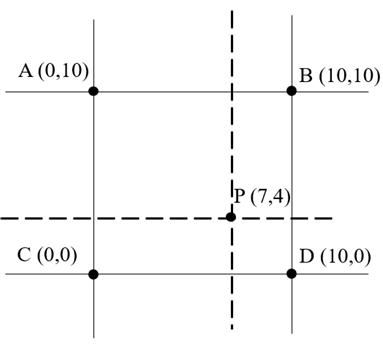
\includegraphics[width=0.5\textwidth]{figs/qn84.png}
    \caption{Diagram}
\label{fig:qn84}
\end{figure}
\end{document}
